
\chapter{Hardware Architecture}

\section{Overview}

This DLX is a 32-bit RISC processor with a five-stage pipeline. \newline
The external interface is made mainly for memories connection (IRAM, DRAM and a DRAM for the Register File), and for the Clock and Reset signals. Inside we find the following blocks:

\begin{itemize}
    \item Control Unit: it receives the fetched instruction from the IR register and starts to output the correct control signals towards all the pipeline stages. Moreover, it receives status signals from all other units about their working status like the comparator result (for branch decision), the status about possible hazards in the pipeline, Register File's Push \& Pop operations under execution, and all the memories readiness. It's in charge of controling the entire pipeline and stop it in case of hazards or other situations that requires a stall.
    \item Decode Unit: part of the decode stage, it is in charge of keeping the status about all registers under use (for further hazard controls), computation of the new Program Counter (given a Jump or not), data comparison (for branches) and, the most important thing, the operation decode with the dispatch of all the operands towards the right ports of the DataPath.
    \item DataPath: the computational core of the processor. Made of 4 pipeline stages (Instruction Decode, Execution, Memory, Write Back) contains all the units capable of doing computation. In particular, we have the Register File (that manages all the registers of the core), the Arithmetic Logic Unit, the Load-Store Unit for data memory management, and other units useful for the correct operation of everything.
    \item IR and PC: two registers the compose the Instruction Fetch stage of the pipeline, they are in charge of keeping in memory the current instruction under execution and the address for the next instruction to execute, respectively. 
\end{itemize}


\begin{figure}[ht]
    \centering
    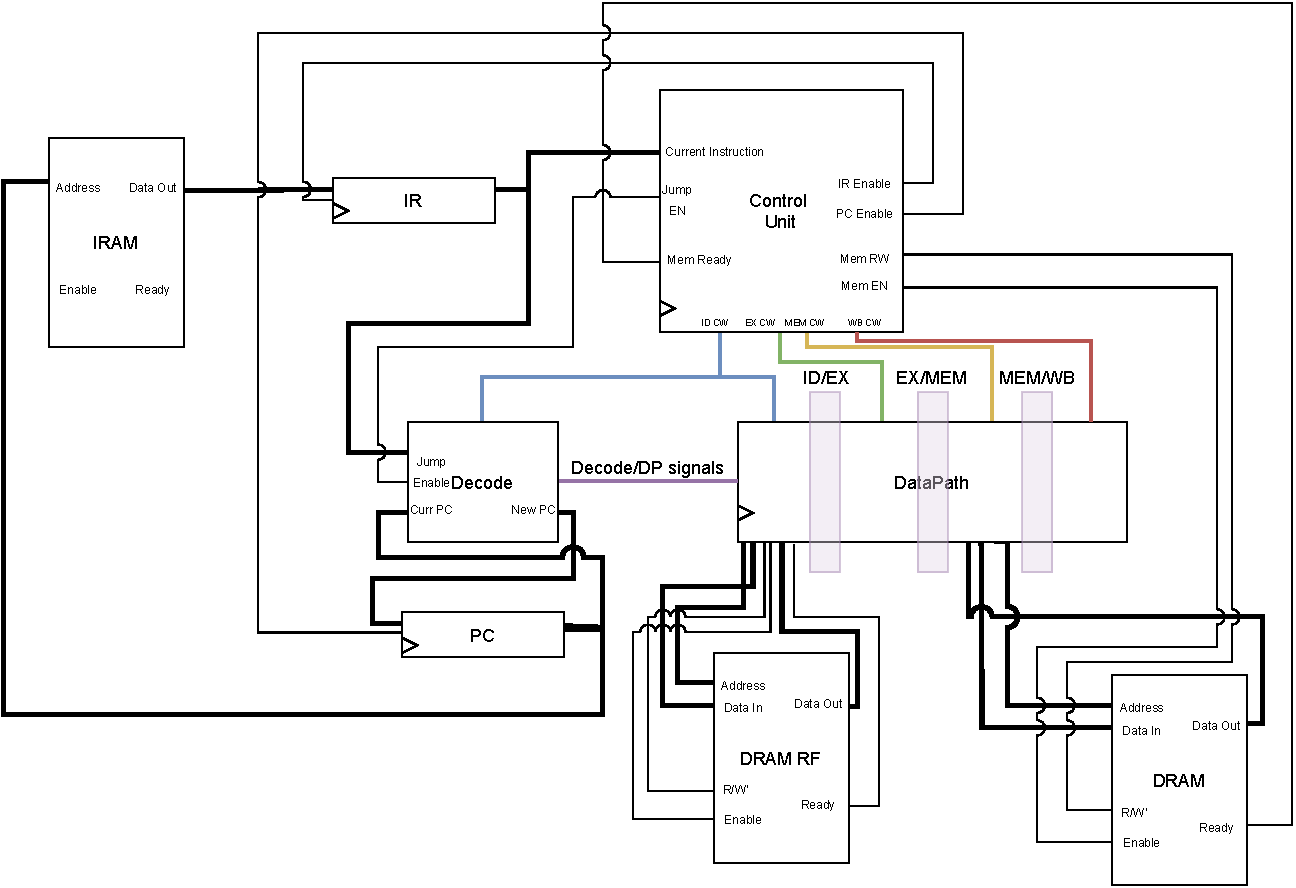
\includegraphics[width=1\textwidth]{chapters/2_dlx/images/DLX.pdf}
    \caption{Schematic of the DLX}
    \label{DLX}
\end{figure} 
\newpage
\section{Pipeline Stages}
\section{Control Unit}
\section{Memory Interface}
\section{Instruction Set}